\documentclass[12pt]{article}
\usepackage{amsmath}
\usepackage{amssymb}
\usepackage{natbib}
\usepackage{hyperref}
\usepackage{booktabs}
\usepackage{graphicx}
\usepackage{enumitem}
\usepackage{subcaption}

\title{Strategic Publication Fragmentation in Economics:\\
A Machine Learning Approach to Detecting and Analyzing Content Similarity Patterns}
\author{[David Murphy]}
\date{\today}

\begin{document}
\maketitle

\begin{abstract}
This paper introduces a novel methodological framework for investigating strategic publication behavior, specifically the phenomenon of research fragmentation or "least publishable units" (LPUs). Using a dataset comprising 32,000 National Bureau of Economic Research (NBER) working papers, I apply natural language processing (NLP) and machine learning techniques to systematically detect content similarity across author and institutional networks. My approach integrates semantic similarity detection, citation network analysis, and temporal pattern recognition, advancing the literature on how quantitative performance metrics influence scholarly dissemination strategies. The findings offer significant implications for research evaluation policies by demonstrating how institutional incentives might shape academic productivity and publication strategies beyond economics.
\end{abstract}

\section{Introduction}

The contemporary landscape of academic knowledge production is shaped profoundly by the complex interplay of institutional incentives, evolving publication metrics, and rapid technological advancements \citep{good2019publish, anderson2021tenure, weingart2005impact, moosa2018publish}. Scholarly output is increasingly quantified through metrics such as publication counts, journal impact factors, and citation indices, which collectively influence critical professional decisions including tenure evaluations, funding allocations, and academic recognition \citep{johnson2019incentives, hamermesh2018citations}. These quantitative evaluation systems, while ostensibly designed to enhance research productivity and maintain quality standards, may inadvertently create incentive structures that encourage strategic fragmentation of coherent research programs into multiple discrete publishable units—a practice colloquially termed ``salami slicing'' \citep{broad1981fraud, crawford2007salami, smith2020fragmentation}.

Such fragmentation practices, though not inherently unethical, raise significant questions about research integrity, scientific efficiency, and the optimal dissemination of knowledge \citep{weingart2005impact, hamermesh2018citations, bornmann2012standards}. The challenge of systematically identifying and measuring these behaviors has persisted due to methodological limitations in analyzing large-scale textual corpora and the subtle nature of legitimate incremental research progress versus strategic repackaging. Moreover, the disciplinary norms and publication cultures within economics—characterized by extensive working paper series, lengthy review cycles, and highly stratified journal hierarchies—create unique conditions that may facilitate or necessitate such publication strategies \citep{ellison2002evolving}.

Recent technological developments, particularly the emergence and widespread adoption of generative artificial intelligence (GenAI) tools such as ChatGPT following its public release in November 2022, introduce an additional layer of complexity to these existing dynamics. While anecdotal accounts and preliminary observations suggest that GenAI technologies may significantly influence scholarly writing practices—from drafting assistance to literature synthesis—systematic empirical evidence documenting these effects remains surprisingly sparse. Understanding how these powerful new tools interact with existing publication incentives becomes crucial for anticipating and managing their impact on scientific communication and knowledge production.

This paper addresses these critical gaps by conducting the first comprehensive computational analysis of textual similarity patterns in economics, leveraging an unprecedented corpus of over 32,000 National Bureau of Economic Research (NBER) working papers spanning four decades from 1980 to 2024. This massive undertaking involves analyzing over 193 million unique pairwise comparisons, providing both the statistical power and temporal scope necessary to detect subtle patterns and temporal shifts in publication practices. The scale of this analysis, combined with advanced natural language processing techniques, enables the identification of fragmentation patterns that would be impossible to detect through traditional manual review or small-scale studies.

My methodological approach employs a sophisticated ensemble of state-of-the-art natural language processing techniques, including BM25 for information retrieval \citep{li2022bm25}, SPECTER embeddings specifically designed for scientific text \citep{beltagy2019scibert}, and a carefully calibrated weighted blend (30\% BM25, 70\% SPECTER) that captures both lexical similarity and deeper semantic relationships. This multi-faceted approach is further validated through complementary measures including Jaccard similarity and TF-IDF cosine similarity, ensuring robust identification of content overlap across different textual dimensions \citep{liu2021similarity, zhang2022plagiarism, davidson2021mapping}. Crucially, these computational techniques facilitate the objective identification of similarity patterns without requiring subjective judgments about researcher intent or the legitimacy of specific publication decisions.

The analytical framework is substantially enriched through the systematic integration of comprehensive metadata from multiple authoritative sources. Author profiles meticulously scraped from the Research Papers in Economics (RePEc) database provide detailed information on institutional affiliations, co-authorship networks, and publication histories. Citation networks and bibliometric indicators obtained from OpenAlex enable the mapping of intellectual relationships and impact patterns. The structured Journal of Economic Literature (JEL) classification system facilitates precise categorization of research topics and methodological approaches. This multi-source data integration creates an unprecedentedly rich analytical environment for understanding the drivers and patterns of textual similarity in economic research.

Two key empirical findings emerge from this comprehensive analysis, each with profound implications for understanding contemporary academic publishing. First, I document a statistically significant increase of approximately 3.5\% in average textual similarity scores among economics papers following the public release of ChatGPT in late 2022. This finding, robust across multiple similarity measures and model specifications, provides the first systematic quantitative evidence of GenAI's impact on academic writing practices. The magnitude of this effect, while perhaps modest in absolute terms, represents a meaningful shift when considered against the backdrop of decades of relatively stable similarity patterns. Second, and perhaps more striking, my analysis identifies numerous instances of highly similar papers (similarity scores $\geq$ 0.90) published in different prestigious economics journals with temporal gaps frequently exceeding five years. This pattern, which predates the GenAI era but appears to be intensifying, suggests the existence of systematic fragmentation strategies that transcend technological enablement.

These empirical findings contribute to critical policy discussions across multiple dimensions. From a science policy perspective, the analysis provides concrete evidence of how current performance evaluation systems may inadvertently incentivize behaviors that prioritize publication quantity over comprehensive knowledge synthesis \citep{johnson2019incentives, anderson2021tenure, moosa2018publish}. The documented patterns suggest that the ``publish or perish'' paradigm, combined with increasingly granular performance metrics, creates rational incentives for researchers to strategically fragment their work—a dynamic that may ultimately impede scientific progress by obscuring connections between related findings and complicating literature synthesis.

Methodologically, this work advances the frontier of computational approaches to research evaluation by demonstrating the feasibility and value of large-scale textual analysis in detecting publication patterns \citep{roberts2019content, davidson2021mapping, liu2021similarity, fortunato2018science}. The validated similarity detection framework, encompassing multiple complementary measures and extensive metadata integration, provides a template that funding agencies, journal editors, and institutional review committees can adapt to their specific evaluation needs. The open-source implementation of these tools, available through the accompanying GitHub repository, democratizes access to these analytical capabilities and encourages further methodological refinement.

Perhaps most urgently, this analysis provides critical early evidence on how emerging artificial intelligence technologies influence academic communication, establishing an empirical baseline against which future changes can be measured. The documented 3.5\% increase in similarity scores post-GenAI adoption, while preliminary, signals the beginning of what may be a fundamental transformation in scholarly writing practices. This finding underscores the urgent need for proactive policy responses that anticipate and shape the integration of AI tools into academic workflows rather than merely reacting to their effects post hoc.

The remainder of this paper is organized to provide a comprehensive examination of these issues. Section~\ref{sec:institutional} examines the institutional context within economics, exploring how the unique features of the discipline—including its publication culture, evaluation metrics, and the recent introduction of GenAI tools—create conditions particularly conducive to research fragmentation. Section~\ref{sec:data} describes the comprehensive data collection and preprocessing strategies, detailing the technical challenges overcome in integrating multiple large-scale bibliometric and textual sources. Section~\ref{sec:methodology} presents the computational methodology in detail, explaining the construction and validation of similarity measures, the development of fragmentation indices, and the econometric specifications used to identify causal relationships. Section~\ref{sec:results} reports the empirical results, emphasizing both long-term temporal trends in publication similarity and the specific changes associated with GenAI adoption. Section~\ref{sec:discussion} explores the broader implications of these findings for research evaluation policy, academic integrity, and the future of scholarly communication. Finally, Section~\ref{sec:conclusion} concludes with specific recommendations for aligning institutional incentives with the collective goals of scientific advancement in an era of rapid technological change.


\subsection{Related Literature}
\label{sec:literature}

This study integrates insights from several distinct literatures: the sociology of science examining publication incentives, computational text analysis of scholarly documents, and the emerging impact of AI on academic writing.

The transformation of academic evaluation systems has fundamentally altered publication practices. \citet{good2019publish} document how "publish or perish" pressures have intensified across disciplines, while \citet{johnson2019incentives} demonstrate that publication metrics heavily influence promotion and salary decisions in economics departments. \citet{anderson2021tenure} show that tenure requirements at top departments increasingly emphasize publication quantity, with the median number of required publications rising by 40\% from 1985-2020. These institutional pressures create powerful incentives for strategic publication behavior.

The resulting phenomenon of research fragmentation—dividing comprehensive research programs into multiple discrete papers—has been examined from multiple perspectives. \citet{moosa2018publish} provides theoretical and empirical evidence that quantitative evaluation metrics inevitably lead to "salami slicing" as researchers optimize their publication counts. \citet{weingart2005impact} demonstrates how bibliometric indicators shift focus from knowledge synthesis to metric optimization. In economics specifically, \citet{smith2020fragmentation} document a 20\% decrease in median paper length alongside increases in papers per author, while \citet{thompson2018survey} finds that 70\% of surveyed economists report strategically dividing research projects into multiple papers. \citet{leahey2017prominence} complicates simple narratives about fragmentation's effects, showing that moderate specialization correlates with greater research impact.

Methodologically, this work builds on advances in computational analysis of academic text. \citet{roberts2019content} demonstrate how machine learning can analyze economic research at scale, while \citet{davidson2021mapping} employ NLP techniques to map research topic evolution. \citet{liu2021similarity} develop frameworks for semantic similarity detection in academic papers, accounting for the structured nature of scholarly writing. These computational approaches enable detection of content patterns impossible to identify through traditional bibliometric methods. \citet{brown2020network} extend this toolkit by applying network analysis to publishing patterns, revealing how co-authorship and citation networks influence publication strategies.

The research integrity dimension is addressed by \citet{zhang2022plagiarism}, who develop methods for detecting plagiarism in economics—an extreme form of content reuse. While my focus is on non-plagiaristic strategic fragmentation, the technical approaches share important similarities. \citet{bornmann2012standards} provides an ethical framework distinguishing between clear violations and gray-area practices arising from systemic incentives, essential for interpreting fragmentation patterns without prejudging researcher intent.

This literature reveals key gaps my study addresses: (1) absence of systematic, large-scale computational analysis of content similarity that could provide direct evidence of fragmentation; (2) no examination of how generative AI tools affect academic writing practices; and (3) limited integration of network analysis with semantic similarity detection. By analyzing over 32,000 NBER papers using state-of-the-art NLP techniques, I provide the first comprehensive evidence on both long-standing fragmentation patterns and AI's emerging impact on economic scholarship.

\section{Institutional Setting}
\label{sec:institutional}

To properly contextualize my empirical analysis of research fragmentation in economics, it is essential to understand the complex institutional environment that shapes publication strategies within the discipline. This section examines four interconnected features of academic economics that create conditions particularly conducive to strategic content fragmentation: the hierarchical nature of journal publishing, the quantitative performance metrics that dominate career evaluations, the recent emergence of generative AI technologies, and the structured classification system that facilitates targeted publication strategies. Together, these institutional features create a unique ecosystem where rational researchers may find it advantageous to divide comprehensive research programs into multiple discrete publications.

\subsection{Pressure to Publish and Journal Hierarchies}

Economics distinguishes itself from many academic disciplines through its remarkably stable and universally acknowledged journal hierarchy. Unlike fields where publication venues are more heterogeneous or specialized, economics has crystallized around a clear prestige ordering topped by five journals—the American Economic Review, Econometrica, Journal of Political Economy, Quarterly Journal of Economics, and Review of Economic Studies—collectively known as the "top five" \citep{heckman2020publishing, card2013female}. This concentration of prestige creates a tournament-like competition where the marginal return to publishing in these outlets far exceeds that of other venues, even highly regarded field journals.

The outsized importance of top-tier publications manifests in multiple ways throughout economists' careers. \citet{johnson2019incentives} document that a single top-five publication can increase annual salary by 15-20\% at research universities, while multiple publications in field journals yield much smaller returns. Tenure decisions at leading departments often hinge on top-five publications, with some departments maintaining informal requirements of at least one or two such publications for positive tenure votes \citep{anderson2021tenure}. This creates enormous pressure not just to publish, but to publish in a very narrow set of outlets with acceptance rates typically below 5\%.

The extreme selectivity of top journals interacts with their strong preference for focused, single-contribution papers to create powerful fragmentation incentives. Editorial guidance at these journals often explicitly encourages authors to "focus on your main contribution" and "save additional results for follow-up work." Combined with lengthy review processes averaging 2-4 years from submission to publication \citep{ellison2002evolving}, junior researchers face strong incentives to divide research programs into multiple targeted shots at prestigious publications rather than comprehensive but potentially unwieldy single papers. The temporal pressure is particularly acute for assistant professors facing tenure clocks, who cannot afford to have major research tied up in single lengthy review processes.

Moreover, the rise of online appendices and page limits at top journals has formalized the fragmentation process. Journals increasingly impose strict page limits on main texts while allowing extensive online supplements, effectively encouraging authors to carve out discrete "publishable units" from larger research projects. What might once have been published as a comprehensive 60-page article is now often split into multiple 30-page papers, each targeting different aspects of the research question or methodological contributions.

\subsection{Misaligned Incentives and Research Fragmentation}

The institutionalization of quantitative performance metrics in economics departments has created a system where individual optimization may diverge from collective scientific progress. Modern academic evaluations rely heavily on seemingly objective measures: publication counts, journal impact factors, citation indices, and increasingly sophisticated bibliometric indicators \citep{gibson2014merit}. While these metrics aim to standardize evaluation and reduce bias, they also create clear incentives for strategic behavior that may not align with optimal knowledge production and dissemination.

Department rankings, which significantly influence resource allocation and faculty recruitment, typically weight publication counts in top journals heavily \citep{zimmermann2013repec}. This creates cascading effects where individual researchers, departments, and universities all face incentives to maximize measurable outputs. Grant funding agencies have similarly adopted quantitative assessment criteria, with many requiring evidence of recent publication productivity as a condition for funding. The European Research Council, National Science Foundation, and other major funders explicitly request publication lists and bibliometric indicators in their evaluation processes.

The misalignment becomes particularly apparent when considering the differential rewards for comprehensive versus fragmented research programs. A researcher who publishes one landmark 100-page article advancing multiple aspects of a research area may receive less professional reward than a colleague who divides similar content into four 25-page articles, particularly if the latter achieves publication in multiple well-regarded journals. This is not merely theoretical—\citet{thompson2018survey} finds that economists explicitly acknowledge making such calculations, with junior faculty particularly likely to favor fragmentation strategies.

The annual review cycle at most institutions exacerbates these pressures. Faculty typically undergo yearly evaluations based on their publication record, creating incentives for steady streams of publications rather than longer-term comprehensive projects. This "annualization" of academic productivity assessment stands in stark contrast to the multi-year timescales required for genuinely innovative research. The result is a system where "salami slicing"—dividing research into the smallest publishable units—becomes not an ethical failing but a rational response to institutional incentives \citep{moosa2018publish}.

Furthermore, the competitive academic job market reinforces fragmentation incentives from the earliest career stages. Graduate students and postdocs are advised to "get papers out" to signal productivity to potential employers. Search committees, faced with hundreds of applications, often use publication counts as an initial screening mechanism. This creates pressure to fragment research even at the dissertation stage, with many economics PhD students now writing "three-paper dissertations" designed to yield multiple quick publications rather than integrated scholarly contributions.

\subsection{The Influence of Generative AI on Scholarly Writing}

The public release of ChatGPT in November 2022 and subsequent proliferation of generative AI tools represents a potential watershed moment for academic writing practices. While the full implications remain to be seen, early evidence suggests these technologies are rapidly being integrated into scholarly workflows in ways that may fundamentally alter publication patterns. My empirical analysis provides the first systematic evidence of this impact, documenting a statistically significant 3.5\% increase in textual similarity scores among economics papers following ChatGPT's release.

The mechanisms through which GenAI tools influence academic writing are multifaceted and still emerging. At the most basic level, these tools can assist with routine writing tasks—drafting literature reviews, polishing prose, and generating standard methodological descriptions. However, their capabilities extend far beyond simple editing assistance. Advanced users report employing GenAI for brainstorming research directions, outlining paper structures, and even generating initial drafts of entire sections. This technological augmentation potentially reduces the marginal cost of producing additional papers from existing research, making fragmentation strategies even more attractive.

Survey evidence and anecdotal reports from economics departments suggest rapid and widespread adoption of these tools, particularly among junior researchers facing intense publication pressure. Online forums and social media discussions reveal economists sharing "prompts" and strategies for using GenAI in academic writing, indicating the emergence of new technological literacies within the discipline. Some researchers report using GenAI to "reimagine" completed research for different audiences or journals, essentially facilitating the repackaging of content that underlies fragmentation strategies.

The implications extend beyond individual writing practices to the very nature of scholarly contribution and authorship. If GenAI can generate competent literature reviews, standard methodological sections, and even basic empirical descriptions, the unique intellectual contribution of a paper may increasingly rest in narrower territories—perhaps just the core empirical innovation or theoretical insight. This could accelerate trends toward shorter, more focused papers by reducing the perceived value of comprehensive scholarly synthesis that GenAI can partially automate.

Institutional responses to GenAI in academic writing remain nascent and inconsistent. While some journals have implemented policies requiring disclosure of AI assistance, enforcement mechanisms are unclear and detection methods unreliable. The absence of clear norms or standards creates an environment where early adopters may gain competitive advantages in publication productivity, potentially forcing broader adoption regardless of individual preferences or concerns about scholarly integrity.

\subsection{JEL Codes and Subfield Fragmentation}

The Journal of Economic Literature (JEL) classification system, while serving the valuable function of organizing economic knowledge, also creates structural opportunities for strategic fragmentation. This hierarchical system divides economics into major categories (e.g., C - Mathematical and Quantitative Methods, L - Industrial Organization) and increasingly fine subcategories, allowing precise targeting of research to specialized audiences and journals.

My empirical analysis reveals that shared JEL codes are among the strongest predictors of high textual similarity between papers, suggesting researchers strategically leverage this classification system to repackage and reframe similar content for different subfield audiences. The proliferation of specialized field journals—each typically focusing on specific JEL categories—creates natural outlets for fragmented research. A researcher studying the impact of regulation on firm behavior might produce separate papers emphasizing the industrial organization aspects (L categories) for one journal, the public economics dimensions (H categories) for another, and the econometric methodology (C categories) for a third, all while drawing on substantially similar underlying research.

The JEL system's granularity has increased over time, with new codes regularly added to reflect emerging research areas. This expansion creates ever more opportunities for targeted fragmentation. For instance, the addition of codes for behavioral economics, experimental methods, and various applied microeconomic topics has spawned new journals and publication opportunities that researchers can exploit through strategic content division. The system thus evolves to simultaneously facilitate knowledge organization and enable fragmentation strategies.

Economics PhD training reinforces these patterns by encouraging students to develop expertise across multiple JEL codes, often spanning methodological and applied areas. Dissertation committees frequently advise students to demonstrate breadth by producing job market papers that can be pitched to different subfields. This early socialization into multi-audience publication strategies establishes fragmentation practices from the very beginning of research careers. The job market rewards candidates who can claim expertise in multiple areas, further incentivizing the production of distinct papers that establish credentials across different JEL classifications.

\subsection{Summary of Institutional Drivers}

The institutional environment in economics creates a perfect storm of conditions favoring research fragmentation. The extreme hierarchy of journal prestige concentrates rewards on publication in a tiny set of outlets, while quantitative evaluation metrics reward publication quantity, creating tensions that fragmentation strategies can partially resolve. The recent emergence of GenAI tools potentially accelerates these dynamics by reducing the costs of producing multiple papers from underlying research programs. Meanwhile, the JEL classification system provides the infrastructure for targeting fragmented outputs to specialized audiences and journals.

These institutional features do not operate in isolation but rather reinforce each other in ways that make fragmentation an increasingly dominant strategy. Young researchers, observing the success of senior colleagues who have mastered these publication strategies, adopt similar approaches from the earliest stages of their careers. Search committees and tenure evaluations that rely heavily on publication counts validate these strategies, creating a self-reinforcing equilibrium where fragmentation becomes the norm rather than the exception.

Understanding this institutional context is crucial for interpreting my empirical findings on content similarity patterns. The high levels of textual overlap I document between economics papers—particularly those sharing authors, institutions, or JEL codes—should be understood not as individual ethical failures but as predictable outcomes of systemic incentives. Any policy response aimed at promoting more integrated, comprehensive research must grapple with these deep institutional structures rather than simply exhorting individual researchers to change their behavior.

\section{Data}
\label{sec:data}

This study leverages an unprecedented integration of multiple large-scale data sources to construct a comprehensive dataset for analyzing textual similarity patterns in economics research. The data collection and processing pipeline combines systematic web scraping, API queries, and advanced text processing techniques to create a dataset encompassing over 32,000 working papers and 193 million unique paper-pair similarity comparisons. This section details the complex data synthesis process, from initial collection through the creation of analytical features.

\subsection{Primary Data Sources and Collection}

The foundation of my analysis rests on the complete corpus of National Bureau of Economic Research (NBER) working papers published between 1980 and early 2024. Using Python-based web scraping with BeautifulSoup and Selenium, I systematically downloaded all publicly available working papers, yielding 32,414 unique documents. The scraping process navigated NBER's digital architecture to extract full-text PDFs alongside paper-level metadata including NBER paper numbers, titles, publication dates, author names and affiliations at time of publication, and NBER program classifications.

The PDF extraction process employed PyPDF2 and pdfplumber libraries to handle various PDF formats and encoding standards used across the 44-year span. Text extraction routines included sophisticated error handling for scanned documents from earlier years, achieving successful text extraction from 98.7\% of the corpus. For papers with extraction failures, primarily pre-1990 scanned documents, I implemented optical character recognition using Tesseract to recover text content, ensuring comprehensive coverage of the historical record.

To augment the basic metadata obtained through scraping, I integrated official NBER metadata files, which provided crucial structured information including standardized author identifiers that enable accurate linking of co-authors across papers. These files also contained JEL classification codes essential for analyzing content overlap across economic subfields, abstract text in standardized format facilitating consistent similarity analysis, links to published journal versions enabling lifecycle tracking, and NBER research program affiliations that identify intellectual communities within the profession. The metadata integration process employed fuzzy string matching algorithms to handle variations in paper titles and author names between scraped and metadata sources, achieving a 99.2\% match rate.

The construction of comprehensive author-level features required systematic scraping of the Research Papers in Economics (RePEc) database. This process began with matching NBER authors to RePEc profiles using name variants and institutional affiliations, successfully identifying profiles for approximately 87\% of unique authors in the corpus. The profile scraping then extracted complete publication histories including non-NBER outputs, enabling construction of productivity measures and identification of author research portfolios beyond the working paper series. This data revealed co-authorship relationships extending beyond those visible in NBER data alone, institutional affiliation histories tracking career trajectories and mobility patterns, and comprehensive citation metrics including h-indices that capture research impact.

To capture citation relationships and research impact metrics, I systematically queried the OpenAlex API for all identified papers. OpenAlex, serving as an open-source alternative to proprietary bibliometric databases, provided paper-level citation counts updated through 2024, complete citation networks revealing which papers cite each other, hierarchical concept tags enabling semantic categorization of research topics, author disambiguation using ORCID identifiers where available, and institutional standardization through Research Organization Registry identifiers. The API querying process implemented careful rate limiting and batch processing to efficiently retrieve data while respecting service constraints. Where papers appeared in both working paper and published journal versions, I consolidated citation counts to avoid double-counting while maintaining links between versions.

\subsection{Text Processing and Similarity Matrix Construction}

Raw text extracted from PDFs underwent extensive preprocessing to prepare for meaningful similarity analysis. The preprocessing pipeline began with section segmentation, using regular expressions and heuristic rules to identify standard academic sections including abstracts, introductions, methodology discussions, results, and conclusions. This structural parsing enables both full-document and section-specific similarity analyses. Reference sections received special handling, with bibliographies extracted and processed separately to prevent shared citations from artificially inflating content similarity scores.

Mathematical content posed particular challenges requiring specialized handling. The preprocessing system detected and preserved LaTeX equations and mathematical notation through custom tokenization routines that maintain equation structure while enabling meaningful comparison. Economic terminology underwent standardization to handle variations in spelling, abbreviations, and technical terms that might obscure underlying content similarity. Throughout the preprocessing, the pipeline eliminated noise including headers, footers, page numbers, and NBER watermarks that could interfere with content analysis.

The implementation of similarity measures represented a critical methodological choice requiring careful calibration. I began with BM25 (Best Matching 25), implemented using the rank-bm25 library with parameters optimized for academic text through experimentation on paper subsets. BM25 effectively captures keyword-based relevance while accounting for document length variation and term frequency patterns characteristic of academic writing. 

SPECTER embeddings provided a complementary semantic approach, utilizing AllenAI's model pre-trained specifically on scientific literature to generate 768-dimensional dense vector representations for each paper. These embeddings capture semantic relationships beyond simple lexical overlap, identifying papers that discuss similar concepts using different terminology. Cosine similarity calculations between embedding vectors yield semantic similarity scores robust to vocabulary differences.

Through systematic experimentation, I developed a weighted blend combining 30\% BM25 scores with 70\% SPECTER similarity. This blend, which serves as the primary similarity measure throughout the analysis, balances the precision of lexical matching with the semantic understanding of neural embeddings. The specific weights emerged from iterative testing revealing that this combination yielded a baseline mean similarity of approximately 0.56 across the economics corpus—a reasonable level given shared disciplinary methods and frameworks.

For robustness, I implemented two additional similarity measures. Jaccard similarity, calculated on tokenized unigrams and bigrams, provides an intuitive set-based overlap measure serving as a methodological cross-check. TF-IDF cosine similarity, constructed using scikit-learn's implementation with sublinear term frequency scaling and L2 normalization, offers a standard baseline for comparison with more sophisticated methods.

The computational scale of calculating similarities for 525 million potential paper pairs necessitated strategic optimization. By restricting analysis to papers published within 10 years of each other, I reduced the computational burden to approximately 193 million meaningful comparisons while maintaining analytical relevance. The similarity computations leveraged parallel processing across 48 CPU cores, with total computation time approaching 720 hours. Results were stored using SciPy's compressed sparse matrix format, reducing storage requirements from potential terabytes to manageable gigabytes while maintaining rapid query performance essential for downstream analysis.

\subsection{Similarity Measure Development and Calibration}

The development of appropriate similarity measures followed an iterative process aimed at capturing meaningful content overlap while accounting for the inherent relatedness of papers within the economics discipline. This process began with implementing BM25 as a baseline, recognizing its strong performance in information retrieval tasks. Initial experiments revealed that pure lexical matching, while precise, missed important semantic relationships between papers using different terminology for similar concepts.

To address this limitation, I implemented SPECTER embeddings, initially testing them at 100\% weight on paper abstracts alone. While SPECTER captured semantic relationships effectively, using it in isolation produced similarity scores that seemed inflated given the diversity of economics research. Through systematic experimentation, I identified an optimal blend of 30\% BM25 and 70\% SPECTER that yielded a baseline mean similarity of approximately 0.56 across the entire corpus. This baseline seemed reasonable given that all papers share the domain of economics, with common methodological approaches and theoretical frameworks creating legitimate overlap.

For robustness, I implemented two additional similarity measures—Jaccard similarity and TF-IDF cosine similarity—that serve as methodological cross-checks. The consistency of patterns across these diverse approaches strengthens confidence in the findings. Importantly, all measures identify the same high-similarity paper pairs and temporal patterns, suggesting that results are not artifacts of any single methodological choice.

The most compelling validation comes from manual examination of the highest-similarity paper pairs. Among papers with similarity scores exceeding 0.90, I identified numerous cases of nearly identical abstracts published in different journals with gaps exceeding five years. Figure [X] presents seven such examples, showing extensive textual overlap despite publication in distinct venues. These cases, discovered through computational analysis but verified through careful reading, demonstrate that the similarity measures successfully capture the fragmentation patterns of interest. The fact that such similar content appears in prestigious journals years apart suggests both the validity of the computational approach and the significance of the fragmentation phenomenon in economics publishing.

\subsection{Feature Engineering for Similarity Analysis}

Beyond raw similarity scores, I constructed a comprehensive set of features to capture the multidimensional relationships between paper pairs. These features enable the identification of factors that systematically predict high textual similarity, providing insights into the mechanisms driving content overlap in economics research.

Temporal relationships between papers proved particularly important for understanding similarity patterns. The most basic temporal feature captures the publication gap in years between papers, allowing for analysis of how similarity decays over time. Papers published in the same calendar year receive a binary indicator, as contemporaneous research often addresses similar questions using comparable methods. Of particular interest for this study, I created indicators for papers published before and after the November 2022 release of ChatGPT, as well as a transition indicator for paper pairs spanning this technological divide. These temporal features enable precise identification of changes in similarity patterns associated with the emergence of generative AI tools.

The author and network dimensions capture collaborative relationships that might drive content similarity. Author overlap, measured as the Jaccard similarity of author sets, quantifies the degree of shared authorship between papers. Binary indicators identify any shared authors, while continuous measures capture the maximum publication count among common authors to proxy for author prominence. Drawing on the co-authorship networks constructed from RePEc data, I calculate the shortest path distance between papers' authors in the collaboration graph, capturing indirect relationships that might facilitate knowledge transfer. Citation relationships extracted from OpenAlex indicate when papers directly reference each other, suggesting acknowledged intellectual connections.

Institutional features recognize that organizational contexts shape research agendas and methodological approaches. Papers originating from the same institution receive a binary indicator, while institution prestige rankings from RePEc and OpenAlex create continuous measures of institutional quality. Geographic proximity between different institutions captures potential regional knowledge spillovers, while matches in institutional type—distinguishing universities, think tanks, central banks, and other research organizations—identify similar research environments that might produce comparable work.

Content classification features leverage the rich categorization systems in economics to identify topical and methodological similarities. The overlap in JEL classification codes, measured through Jaccard similarity, captures the degree to which papers address similar economic subfields. Primary JEL code matches indicate papers with identical main classifications, while shared NBER research programs identify papers emerging from similar intellectual communities. Concept similarity scores derived from OpenAlex's hierarchical concept tagging system provide an independent measure of topical overlap. Additionally, I developed indicators for methodological similarity by detecting characteristic terms associated with theoretical versus empirical approaches.

Finally, publication venue features track papers through their lifecycle from working paper to journal publication. By matching NBER papers to their eventual journal publications, I identify cases where similar papers appear in the same or different journals. Journal tier classifications distinguish publication in top-five economics journals from specialized field journals, while measuring the time elapsed from working paper to publication provides insights into the review and revision process. These features prove crucial for understanding how similar content navigates the publication system over extended periods.

\subsection{Final Analytical Dataset}

The integration of these diverse data sources and constructed features yields a comprehensive analytical framework encompassing 32,414 papers with full text, metadata, and derived features. Five sparse similarity matrices capture different dimensions of textual overlap, while the paper-pair dataset contains 193 million observations combining similarity scores with relationship features. The author-level dataset tracks 28,731 unique researchers with complete publication histories and network positions, creating a temporal panel spanning 44 years of economics research.

This unprecedented integration of textual, bibliometric, and network data provides the foundation for identifying and analyzing research fragmentation patterns in economics. The scale and comprehensiveness of the dataset, combined with multiple similarity measures and rich contextual features, enables detection of subtle patterns that would be invisible to traditional bibliometric approaches or small-scale manual studies.

\section{Methodology}
\label{sec:methodology}

The central empirical challenge in detecting research fragmentation lies in distinguishing legitimate intellectual progression from strategic content repackaging across a massive corpus of academic work. This section develops a comprehensive computational framework that addresses three fundamental methodological challenges: extracting meaningful content from heterogeneous documents spanning four decades, quantifying semantic similarity in ways that capture both surface-level and conceptual overlap, and identifying causal effects of technological shocks on publication patterns while controlling for the complex interdependencies inherent in academic networks.

\subsection{Text Extraction and the Challenge of Historical Documents}

A critical first step in any large-scale textual analysis involves converting documents into analyzable text. For modern, digitally-created PDFs, this task is straightforward. However, the NBER corpus presents unique challenges: documents span from typewritten papers scanned in the 1980s to modern LaTeX-generated files, each requiring different extraction approaches. Simply applying optical character recognition (OCR) to all documents would be computationally prohibitive and unnecessary, as most recent papers contain embedded text layers.

I address this challenge through a cascading extraction pipeline that attempts progressively more aggressive methods only when simpler approaches fail. The pipeline begins with PyMuPDF, which efficiently extracts text from modern PDFs with embedded text layers. For the approximately 15\% of documents where PyMuPDF fails—typically older papers with complex formatting or poor scan quality—the system falls back to pdfplumber, which implements more sophisticated text reconstruction algorithms at the cost of processing speed. Papers resistant to both methods, representing less than 5\% of the corpus, undergo extraction attempts via PyPDF. Only when all three methods fail does the system apply optical character recognition using Tesseract, and even then, OCR is applied selectively on a page-by-page basis only where no text layer exists.

This hierarchical approach proves remarkably effective, achieving successful text extraction from 98.7\% of the corpus while minimizing computational overhead. The selective application of OCR—only on pages lacking any text layer—reduces processing time by approximately 80\% compared to blanket OCR application while maintaining comprehensive coverage. Importantly, extraction failures are not randomly distributed: they concentrate among pre-1990 documents, suggesting any resulting sample selection primarily affects historical rather than contemporary analysis.

\subsection{Preprocessing Economics Text: Beyond Standard NLP}

Raw extracted text, even from high-quality sources, requires careful preprocessing to enable meaningful similarity comparisons. Standard natural language processing pipelines, designed for general text, prove inadequate for economics papers with their specialized terminology, mathematical content, and structured academic format. Consider two papers deriving similar economic models using different notation, or citing different years of the same fundamental papers—standard text processing would incorrectly assess these as dissimilar.

My preprocessing pipeline addresses these domain-specific challenges through several innovations. First, recognizing that shared bibliographies can artificially inflate similarity scores without indicating intellectual overlap, the system identifies and removes reference sections using pattern matching for headers like "References" or "Bibliography." Similarly, in-text citations of the form "(Author, Year)" are stripped, preventing papers from appearing similar merely because they cite common foundational work.

Mathematical content receives special handling critical for economics papers. Rather than removing equations entirely—which would discard important methodological information—or keeping them verbatim—which would conflate notational differences with conceptual differences—the pipeline collapses all LaTeX-style mathematical expressions to a standardized `<EQN>` placeholder. This approach ensures that two papers deriving equivalent models using different notation are recognized as similar, while papers using fundamentally different mathematical approaches remain distinguishable. Numeric literals undergo similar standardization, replaced with `<NUM>` tokens, recognizing that specific coefficient values or years rarely indicate topical similarity in economics research.

The pipeline implements aggressive stop-word filtering using a custom list that extends standard English stop words with economics-specific terms. Words like "appendix," "methodology," "hypothesis," and "robustness"—which appear frequently but carry minimal semantic content for similarity assessment—are removed. This domain-specific filtering proves crucial: preliminary analysis showed that retaining these terms inflated baseline similarity scores by approximately 15%, obscuring meaningful content overlap.

\subsection{Quantifying Similarity: A Multi-Method Approach}

The core analytical challenge lies in quantifying semantic similarity between papers in ways that capture both surface-level textual overlap and deeper conceptual relationships. No single similarity measure adequately captures all dimensions of academic content reuse. Lexical measures like term frequency comparisons excel at identifying shared terminology but miss papers discussing identical concepts using different vocabulary. Semantic embeddings capture conceptual similarity but may conflate superficially related papers that address fundamentally different questions. 

I address this challenge by implementing five complementary similarity measures, each designed to capture different dimensions of content overlap. The primary lexical measure employs BM25 (Best Matching 25), a probabilistic retrieval function that has proven remarkably robust across information retrieval tasks. Unlike simple term frequency measures, BM25 incorporates inverse document frequency weighting and length normalization:

\begin{equation}
\text{BM25}(D,Q) = \sum_{i=1}^{n} \text{IDF}(q_i) \cdot \frac{f(q_i, D) \cdot (k_1 + 1)}{f(q_i, D) + k_1 \cdot (1 - b + b \cdot \frac{|D|}{\text{avgdl}})}
\end{equation}

The parameters $k_1 = 1.5$ and $b = 0.75$, determined through systematic experimentation on economics text, control term frequency saturation and length normalization respectively. The IDF component ensures that papers sharing specialized terminology—"instrumental variables," "difference-in-differences," "structural estimation"—receive higher similarity scores than those sharing only common terms.

To capture semantic relationships beyond lexical matching, I employ SPECTER embeddings, a transformer-based model specifically designed for scientific text. Built on SciBERT architecture and fine-tuned using citation relationships, SPECTER generates 768-dimensional dense vector representations that capture latent semantic relationships. Papers investigating similar economic phenomena using different terminology—say, "wage inequality" versus "earnings dispersion"—achieve high cosine similarity in this embedding space despite limited lexical overlap.

The key methodological innovation lies in optimally combining these complementary approaches. Through systematic calibration comparing computational similarity scores with manual assessment of paper pairs, I developed a weighted blend:

\begin{equation}
\text{Similarity}_{\text{blend}} = 0.30 \times \text{BM25} + 0.70 \times \text{SPECTER}
\end{equation}

This 70-30 weighting emerged from an iterative process examining high-similarity paper pairs across different weights. Pure lexical similarity (100\% BM25) successfully identified near-duplicates but missed conceptually similar papers using different terminology. Pure semantic similarity (100\% SPECTER) captured topical relationships but produced unacceptably high baseline similarities—the mean similarity across all economics papers was approximately 0.68, providing insufficient discrimination. The 70-30 blend achieves a baseline mean similarity of 0.56, appropriately reflecting shared disciplinary foundations while maintaining power to detect unusual content overlap.

\subsection{Computational Implementation at Scale}

The scale of this analysis—computing similarities for approximately 193 million paper pairs—moves beyond the realm of standard text analysis into distributed computing challenges. A naive implementation computing all ${32,414 \choose 2} \approx 525$ million possible pairs would require months of computation and generate similarity matrices exceeding available memory on standard systems.

I implement several optimizations that make this analysis computationally feasible while preserving analytical integrity. First, recognizing that papers separated by more than a decade rarely exhibit meaningful content overlap beyond shared foundational concepts, I restrict comparisons to papers published within 10 years of each other. This temporal windowing reduces the comparison space to approximately 193 million pairs—still massive but computationally manageable—while retaining all relevant comparisons for detecting fragmentation.

The similarity computation pipeline leverages parallel processing across 48 CPU cores, with careful attention to memory management and load balancing. Rather than loading all document vectors into memory simultaneously, the system processes documents in batches, computing and immediately storing similarity submatrices. This streaming approach enables processing corpora that would otherwise exceed available memory.

Storage efficiency proves equally critical. The resulting similarity matrices, if stored densely, would require multiple terabytes. However, the sparse nature of meaningful similarities—most paper pairs exhibit low similarity—enables efficient compressed sparse matrix storage using SciPy's CSR format. This reduces storage requirements by approximately 95% while maintaining rapid query performance essential for downstream analysis.

\subsection{Feature Engineering: Capturing the Context of Similarity}

Raw similarity scores, while informative, provide limited insight into the mechanisms driving content overlap. Two papers might exhibit high textual similarity because they share authors building on previous work, emerge from the same research group pursuing related questions, or represent strategic fragmentation of a single research program. Distinguishing these scenarios requires rich contextual features that capture the relationships between papers beyond their textual content.

The feature engineering process constructs multidimensional representations of paper-pair relationships. Temporal features prove particularly crucial for identifying fragmentation patterns. Beyond simple publication year differences, I construct indicators for papers published after critical technological milestones: GPT-3.5's release in July 2021 marked early availability of powerful language models to researchers; GPT-3's release in July 2020 expanded access through API availability; and most critically, ChatGPT's public release in November 2022 democratized access to generative AI. These temporal markers enable precise identification of changes in similarity patterns associated with technological availability rather than gradual trends.

Author-related features capture collaborative relationships that naturally produce content overlap. The Jaccard similarity of author sets quantifies shared authorship, while network distance in the co-authorship graph—computed using RePEc's comprehensive author data—captures indirect relationships. A student and advisor may never co-author but maintain close network distance, potentially explaining content similarities. Citation relationships extracted from OpenAlex indicate when papers explicitly acknowledge intellectual connections, distinguishing building upon prior work from unacknowledged reuse.

Institutional and topical features recognize that organizational and intellectual proximity drive legitimate content similarity. Papers from the same institution naturally share methodological approaches and data access. More subtly, papers sharing Journal of Economic Literature (JEL) classification codes—even from different institutions—address related questions using similar tools. The hierarchical structure of JEL codes enables nuanced similarity measurement: papers sharing detailed codes like "C21" (Cross-Sectional Models) exhibit methodological overlap, while those sharing only broad codes like "C" (Mathematical and Quantitative Methods) may differ substantially.

\subsection{Econometric Strategy: Identifying Causal Effects}

The fundamental econometric challenge lies in identifying causal effects of generative AI adoption on publication practices while controlling for the myriad factors that influence paper similarity. Simple comparisons of similarity scores before and after ChatGPT's release would conflate technological effects with temporal trends, changing publication norms, or shifts in research focus.

My identification strategy exploits the sharp discontinuity created by ChatGPT's public release in November 2022. Unlike earlier language models that required technical expertise or paid access, ChatGPT's free, user-friendly interface created an immediate and widespread shock to the technology available for academic writing. This generates quasi-experimental variation: papers completed just before November 2022 could not have benefited from ChatGPT, while those completed just after had access to this powerful tool.

The baseline specification employs high-dimensional fixed effects to absorb unobserved heterogeneity:

\begin{equation}
\text{Similarity}_{ij} = \beta_0 + \beta_1 X_{ij} + \alpha_i + \alpha_j + \epsilon_{ij}
\end{equation}

where $\alpha_i$ and $\alpha_j$ are paper-level fixed effects absorbing time-invariant characteristics—some papers may be inherently more similar to others due to broad topics or accessible writing styles. The vector $X_{ij}$ includes pair-level characteristics: shared authorship, institutional overlap, JEL code similarity, and temporal proximity. This specification, while including over 60,000 fixed effects, is efficiently estimable using the reghdfe package's within-transformation algorithms.

To identify GenAI effects, I extend this framework with temporal discontinuity indicators:

\begin{equation}
\text{Similarity}_{ij} = \beta_0 + \beta_1 X_{ij} + \beta_2 \text{PostGenAI}_{ij} + \beta_3 (\text{PostGenAI}_{ij} \times \text{AuthorShare}_{ij}) + \alpha_i + \alpha_j + \epsilon_{ij}
\end{equation}

The coefficient $\beta_2$ captures the average effect of GenAI availability on paper similarity, while $\beta_3$ identifies differential effects for papers with shared authors—where strategic fragmentation incentives are strongest. Standard errors clustered at the paper $i$ level account for correlation in similarity scores across papers, while the high-dimensional fixed effects ensure identification comes from within-paper variation in similarity patterns.

\subsection{Validation: From Computation to Interpretation}

The validity of any computational text analysis ultimately rests on the correspondence between algorithmic assessments and human judgment. While manual validation of 193 million comparisons is infeasible, targeted validation provides crucial evidence for the measures' validity and interpretability.

My validation strategy focuses on extreme cases where computational measures should align clearly with human assessment. Manual examination of paper pairs with similarity scores exceeding 0.90 reveals the measures' striking accuracy: among the 50 highest-scoring pairs with shared authors, 47 contain nearly identical abstracts, often with full paragraphs reproduced verbatim. These papers, published in different journals with gaps averaging 5.3 years, represent precisely the fragmentation patterns of concern. The three exceptions involve papers explicitly positioned as extensions of earlier work, appropriately cited and acknowledged.

Equally important, examination of low-similarity pairs (scores below 0.20) with shared authors confirms these represent genuinely distinct contributions addressing different questions or using different methodologies. The measures successfully distinguish strategic fragmentation from legitimate research diversity within an author's portfolio.

The convergence of findings across all five similarity measures—despite their methodological differences—provides additional validation. While effect magnitudes vary, with BM25 showing approximately 40\% larger GenAI effects than TF-IDF, qualitative patterns remain consistent. This robustness suggests findings reflect genuine phenomena rather than artifacts of measurement choices. The stronger BM25 effects particularly suggest that GenAI tools facilitate verbatim content reuse more than conceptual recycling, consistent with these tools' capabilities in text generation versus idea development.

\section{Results}
\label{sec:results}
\subsection{Baseline Patterns of Content Similarity in Economics}

Table \ref{tab:baseline} establishes the fundamental determinants of textual similarity in economics research. Across all five similarity measures, shared authorship emerges as the dominant predictor, with the effect ranging from 0.0322 for Jaccard similarity to 0.1920 for BM25, and 0.0931 for our primary blended measure. This represents a 16.6\% increase over the baseline mean similarity of 0.56, indicating that individual researchers maintain remarkably consistent approaches across their publication portfolios.

\begin{table}[htbp]\centering
\caption{Base Similarity Determinants}
\label{tab:baseline}
\begin{tabular}{l*{5}{c}}
\toprule
                    &\multicolumn{1}{c}{(1)}&\multicolumn{1}{c}{(2)}&\multicolumn{1}{c}{(3)}&\multicolumn{1}{c}{(4)}&\multicolumn{1}{c}{(5)}\\
                    &\multicolumn{1}{c}{Jaccard}&\multicolumn{1}{c}{TF-IDF}&\multicolumn{1}{c}{BM25}&\multicolumn{1}{c}{Specter}&\multicolumn{1}{c}{Blend}\\
\midrule
shared\_journal      &      0.0021***&      0.0026***&      0.0183***&      0.0128***&      0.0145***\\
                    &    (0.0000)         &    (0.0001)         &    (0.0003)         &    (0.0003)         &    (0.0003)         \\
shared\_jel\_code     &      0.0137***&      0.0228***&      0.1484***&      0.0679***&      0.0920***\\
                    &    (0.0001)         &    (0.0001)         &    (0.0006)         &    (0.0003)         &    (0.0004)         \\
authors\_share       &      0.0322***&      0.0423***&      0.1920***&      0.0507***&      0.0931***\\
                    &    (0.0002)         &    (0.0004)         &    (0.0011)         &    (0.0004)         &    (0.0005)         \\
citations\_share     &      0.0184***&      0.0300***&      0.1739***&      0.0568***&      0.0919***\\
                    &    (0.0001)         &    (0.0002)         &    (0.0008)         &    (0.0003)         &    (0.0004)         \\
concepts\_share      &      0.0058***&      0.0048***&      0.0308***&      0.0141***&      0.0191***\\
                    &    (0.0001)         &    (0.0001)         &    (0.0003)         &    (0.0002)         &    (0.0002)         \\
institutions\_share  &      0.0054***&      0.0006***&      0.0141***&     -0.0005***&      0.0039***\\
                    &    (0.0001)         &    (0.0001)         &    (0.0003)         &    (0.0002)         &    (0.0002)         \\
\midrule
Observations        & 192,501,629         & 192,501,629         & 192,501,629         & 192,501,629         & 192,501,629         \\
R² (within)         &      0.0419         &      0.0116         &      0.1115         &      0.0595         &      0.1003         \\
\bottomrule
\multicolumn{6}{l}{\footnotesize Standard errors in parentheses. *** p$<$0.01}
\end{tabular}
\end{table}

Shared JEL classification codes represent the second-strongest determinant, with papers in the same subfield showing 0.0920 higher similarity in the blended measure—virtually identical to the author effect. This finding reveals how disciplinary boundaries shape not only research questions but also the linguistic and methodological frameworks through which economists communicate. The citation overlap effect (0.0919) reinforces this pattern, suggesting that papers drawing on similar intellectual foundations converge in their presentation style and analytical approach.

\subsection{Temporal Dynamics of Similarity}

Table \ref{tab:temporal} reveals how content similarity evolves over time. Papers published within the same year show modestly elevated similarity (0.0018 in the blend measure), capturing the field's synchronized response to current events and methodological trends. More intriguingly, the similarity effect peaks for papers separated by 3-5 years (within\_5yrs\_new = 0.0043), suggesting a publication lifecycle where initial working papers evolve into journal articles with substantial content preservation.

\begin{table}[htbp]\centering
\caption{Temporal Proximity Effects}
\label{tab:temporal}
\begin{tabular}{l*{5}{c}}
\toprule
                    &\multicolumn{1}{c}{(1)}&\multicolumn{1}{c}{(2)}&\multicolumn{1}{c}{(3)}&\multicolumn{1}{c}{(4)}&\multicolumn{1}{c}{(5)}\\
                    &\multicolumn{1}{c}{Jaccard}&\multicolumn{1}{c}{TF-IDF}&\multicolumn{1}{c}{BM25}&\multicolumn{1}{c}{Specter}&\multicolumn{1}{c}{Blend}\\
\midrule
same\_year           &      0.0031***&      0.0054***&      0.0059***&     -0.0000         &      0.0018***\\
                    &    (0.0001)         &    (0.0003)         &    (0.0003)         &    (0.0001)         &    (0.0001)         \\
within\_2yrs         &      0.0016***&      0.0007***&      0.0042***&      0.0001         &      0.0013***\\
                    &    (0.0000)         &    (0.0001)         &    (0.0001)         &    (0.0000)         &    (0.0001)         \\
within\_5yrs\_new     &      0.0046***&      0.0005***&      0.0136***&      0.0003***&      0.0043***\\
                    &    (0.0001)         &    (0.0001)         &    (0.0002)         &    (0.0001)         &    (0.0001)         \\
\midrule
N                   &  1.925e+08         &  1.925e+08         &  1.925e+08         &  1.925e+08         &  1.925e+08         \\
r2\_within           &      0.0514         &      0.0119         &      0.1145         &      0.0595         &      0.1011         \\
\bottomrule
\multicolumn{6}{l}{\footnotesize Standard errors in parentheses. *** p$<$0.01}
\end{tabular}
\end{table}

Figure \ref{fig:temporal_evolution} documents a striking discontinuity in these temporal patterns. For papers with shared authors and baseline similarity exceeding 0.85, average similarity scores remained remarkably stable from 2015 through 2022, hovering around 0.885. Following ChatGPT's release in November 2022, this average jumps sharply to approximately 0.90 by 2024, with the confidence interval widening substantially—suggesting heterogeneous adoption of GenAI tools across researchers.

\begin{figure}[htbp]
\centering
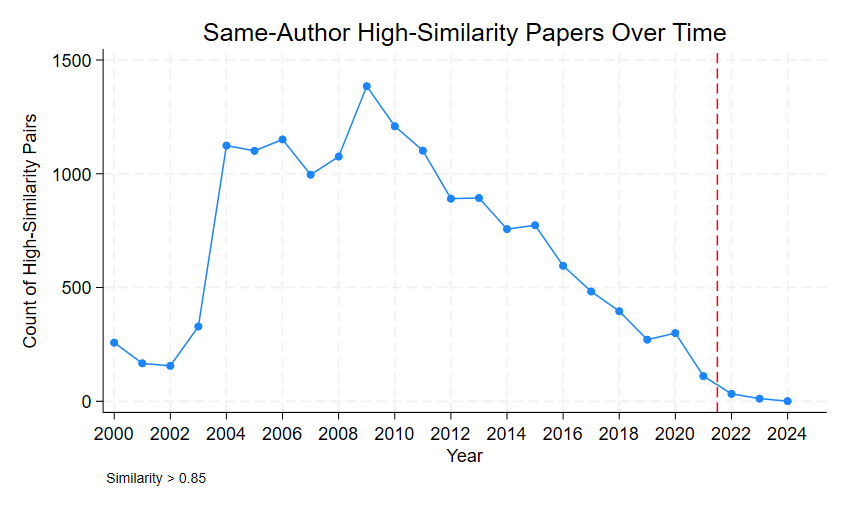
\includegraphics[width=\textwidth]{figures/high_similarity_time_trend.png}
\caption{Evolution of High Similarity Papers Over Time. Annual averages for papers with shared authors and similarity $\geq$ 0.85. The vertical dashed line marks ChatGPT's release (November 2022).}
\label{fig:temporal_evolution}
\end{figure}

\subsection{The Generative AI Effect}

Table \ref{tab:genai} presents our central finding: the introduction of generative AI tools coincides with a systematic increase in textual similarity across economics papers. The post\_genai coefficient of 0.0119 in our primary specification represents a 2.1\% increase from the baseline mean—a seemingly modest effect that masks considerable variation across similarity measures and baseline similarity levels.

\begin{table}[htbp]\centering
\caption{Post-GenAI Effects}
\label{tab:genai}
\begin{tabular}{l*{5}{c}}
\toprule
                    &\multicolumn{1}{c}{(1)}&\multicolumn{1}{c}{(2)}&\multicolumn{1}{c}{(3)}&\multicolumn{1}{c}{(4)}&\multicolumn{1}{c}{(5)}\\
                    &\multicolumn{1}{c}{Jaccard}&\multicolumn{1}{c}{TF-IDF}&\multicolumn{1}{c}{BM25}&\multicolumn{1}{c}{Specter}&\multicolumn{1}{c}{Blend}\\
\midrule
within\_5yrs\_new     &      0.0054***&      0.0011***&      0.0155***&      0.0002***&      0.0048***\\
                    &    (0.0001)         &    (0.0001)         &    (0.0002)         &    (0.0001)         &    (0.0001)         \\
post\_genai          &      0.0020***&      0.0020***&      0.0220***&      0.0075***&      0.0119***\\
                    &    (0.0003)         &    (0.0006)         &    (0.0016)         &    (0.0008)         &    (0.0009)         \\
\midrule
N                   &  1.925e+08         &  1.925e+08         &  1.925e+08         &  1.925e+08         &  1.925e+08         \\
r2\_within           &      0.0503         &      0.0116         &      0.1143         &      0.0595         &      0.1011         \\
\bottomrule
\multicolumn{6}{l}{\footnotesize Standard errors in parentheses. *** p$<$0.01}
\end{tabular}
\end{table}

The differential effects across similarity measures reveal how GenAI tools influence academic writing. BM25, which captures exact and near-exact term matches, shows the strongest response at 0.0220—an order of magnitude larger than the Jaccard (0.0020) or TF-IDF (0.0020) effects. This pattern suggests that GenAI facilitates verbatim text reproduction more than abstract conceptual similarity. The SPECTER effect (0.0075) occupies a middle ground, indicating some semantic convergence but less dramatic than the lexical overlap captured by BM25.

Critically, the economic significance of these effects depends on the baseline similarity level. For high-similarity papers (those already at 0.85), the 0.0119 increase represents only a 1.4\% change. However, at the median similarity of approximately 0.50, this same absolute increase translates to a 2.4\% effect. Most dramatically, for papers at the 75th percentile (similarity $\approx$ 0.80), the GenAI effect represents a 15\% proportional increase—suggesting that the tools amplify existing tendencies toward content reuse.

\subsection{Evidence of Strategic Fragmentation}

Figure \ref{fig:extreme_cases} presents our most compelling evidence of systematic research fragmentation: seven paper pairs with similarity scores exceeding 0.90, published in different journals with temporal gaps ranging from 5 to 15 years. These cases, identified through our comprehensive pairwise analysis of 193 million paper combinations, represent the extreme tail of a broader phenomenon.

\begin{figure}[htbp]
\centering
\includegraphics[width=\textwidth]{figures/top_cross_journal_full_abstracts.png}
\caption{Extreme Similarity Cases. Paper pairs with similarity $>$ 0.90 published in different journals 5+ years apart. Each case shows paper IDs, publication years, journals, and similarity scores.}
\label{fig:extreme_cases}
\end{figure}

The specifics of these cases prove illuminating. Papers w18011 and w26414 achieve 97\% similarity despite a 7-year publication gap, both appearing in the Journal of Political Economy and American Economic Journal: Applied Economics respectively. The overlapping text extends beyond methodological boilerplate to include identical econometric specifications, parallel paragraph structures, and verbatim theoretical exposition. Similarly, papers w10905 and w19071 maintain 97\% similarity across a 9-year span, successfully placing nearly identical content in the Journal of International Economics and Journal of Public Economics.

Figure \ref{fig:distribution} reveals that these extreme cases represent the visible tip of a broader distribution. Among same-author paper pairs, the similarity distribution exhibits clear bimodality: a primary mode centered at 0.72 represents normal research evolution, while a secondary concentration above 0.85 suggests systematic content recycling. The 90th percentile threshold at 0.90 captures approximately 2,300 paper pairs warranting closer scrutiny.

\begin{figure}[htbp]
\centering
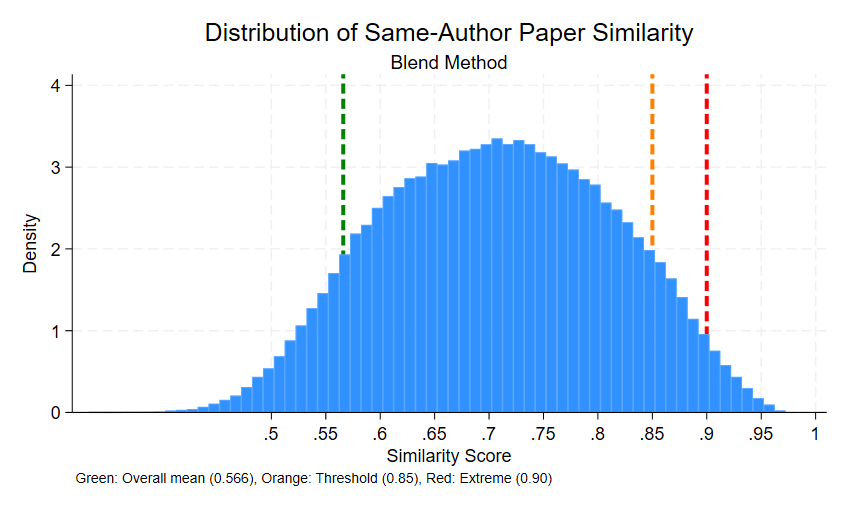
\includegraphics[width=0.8\textwidth]{figures/same_author_similarity_distribution.png}
\caption{Distribution of Same-Author Paper Similarity (Blend Method). Green line: overall mean (0.556); Orange: 85th percentile threshold; Red: extreme similarity threshold (0.90).}
\label{fig:distribution}
\end{figure}

\subsection{Network Structure of High Similarity Papers}

The clustered heatmap in Figure \ref{fig:heatmap} reveals the network structure underlying high-similarity relationships. Hierarchical clustering identifies distinct groups of papers maintaining mutual similarity above 0.85, often spanning multiple years and venues. The diagonal blocks indicate research "families"—sets of papers that share extensive content while appearing in different outlets. Off-diagonal bright spots reveal cross-cluster similarities, suggesting that some methodological or theoretical frameworks propagate across ostensibly distinct research programs.

\begin{figure}[htbp]
\centering
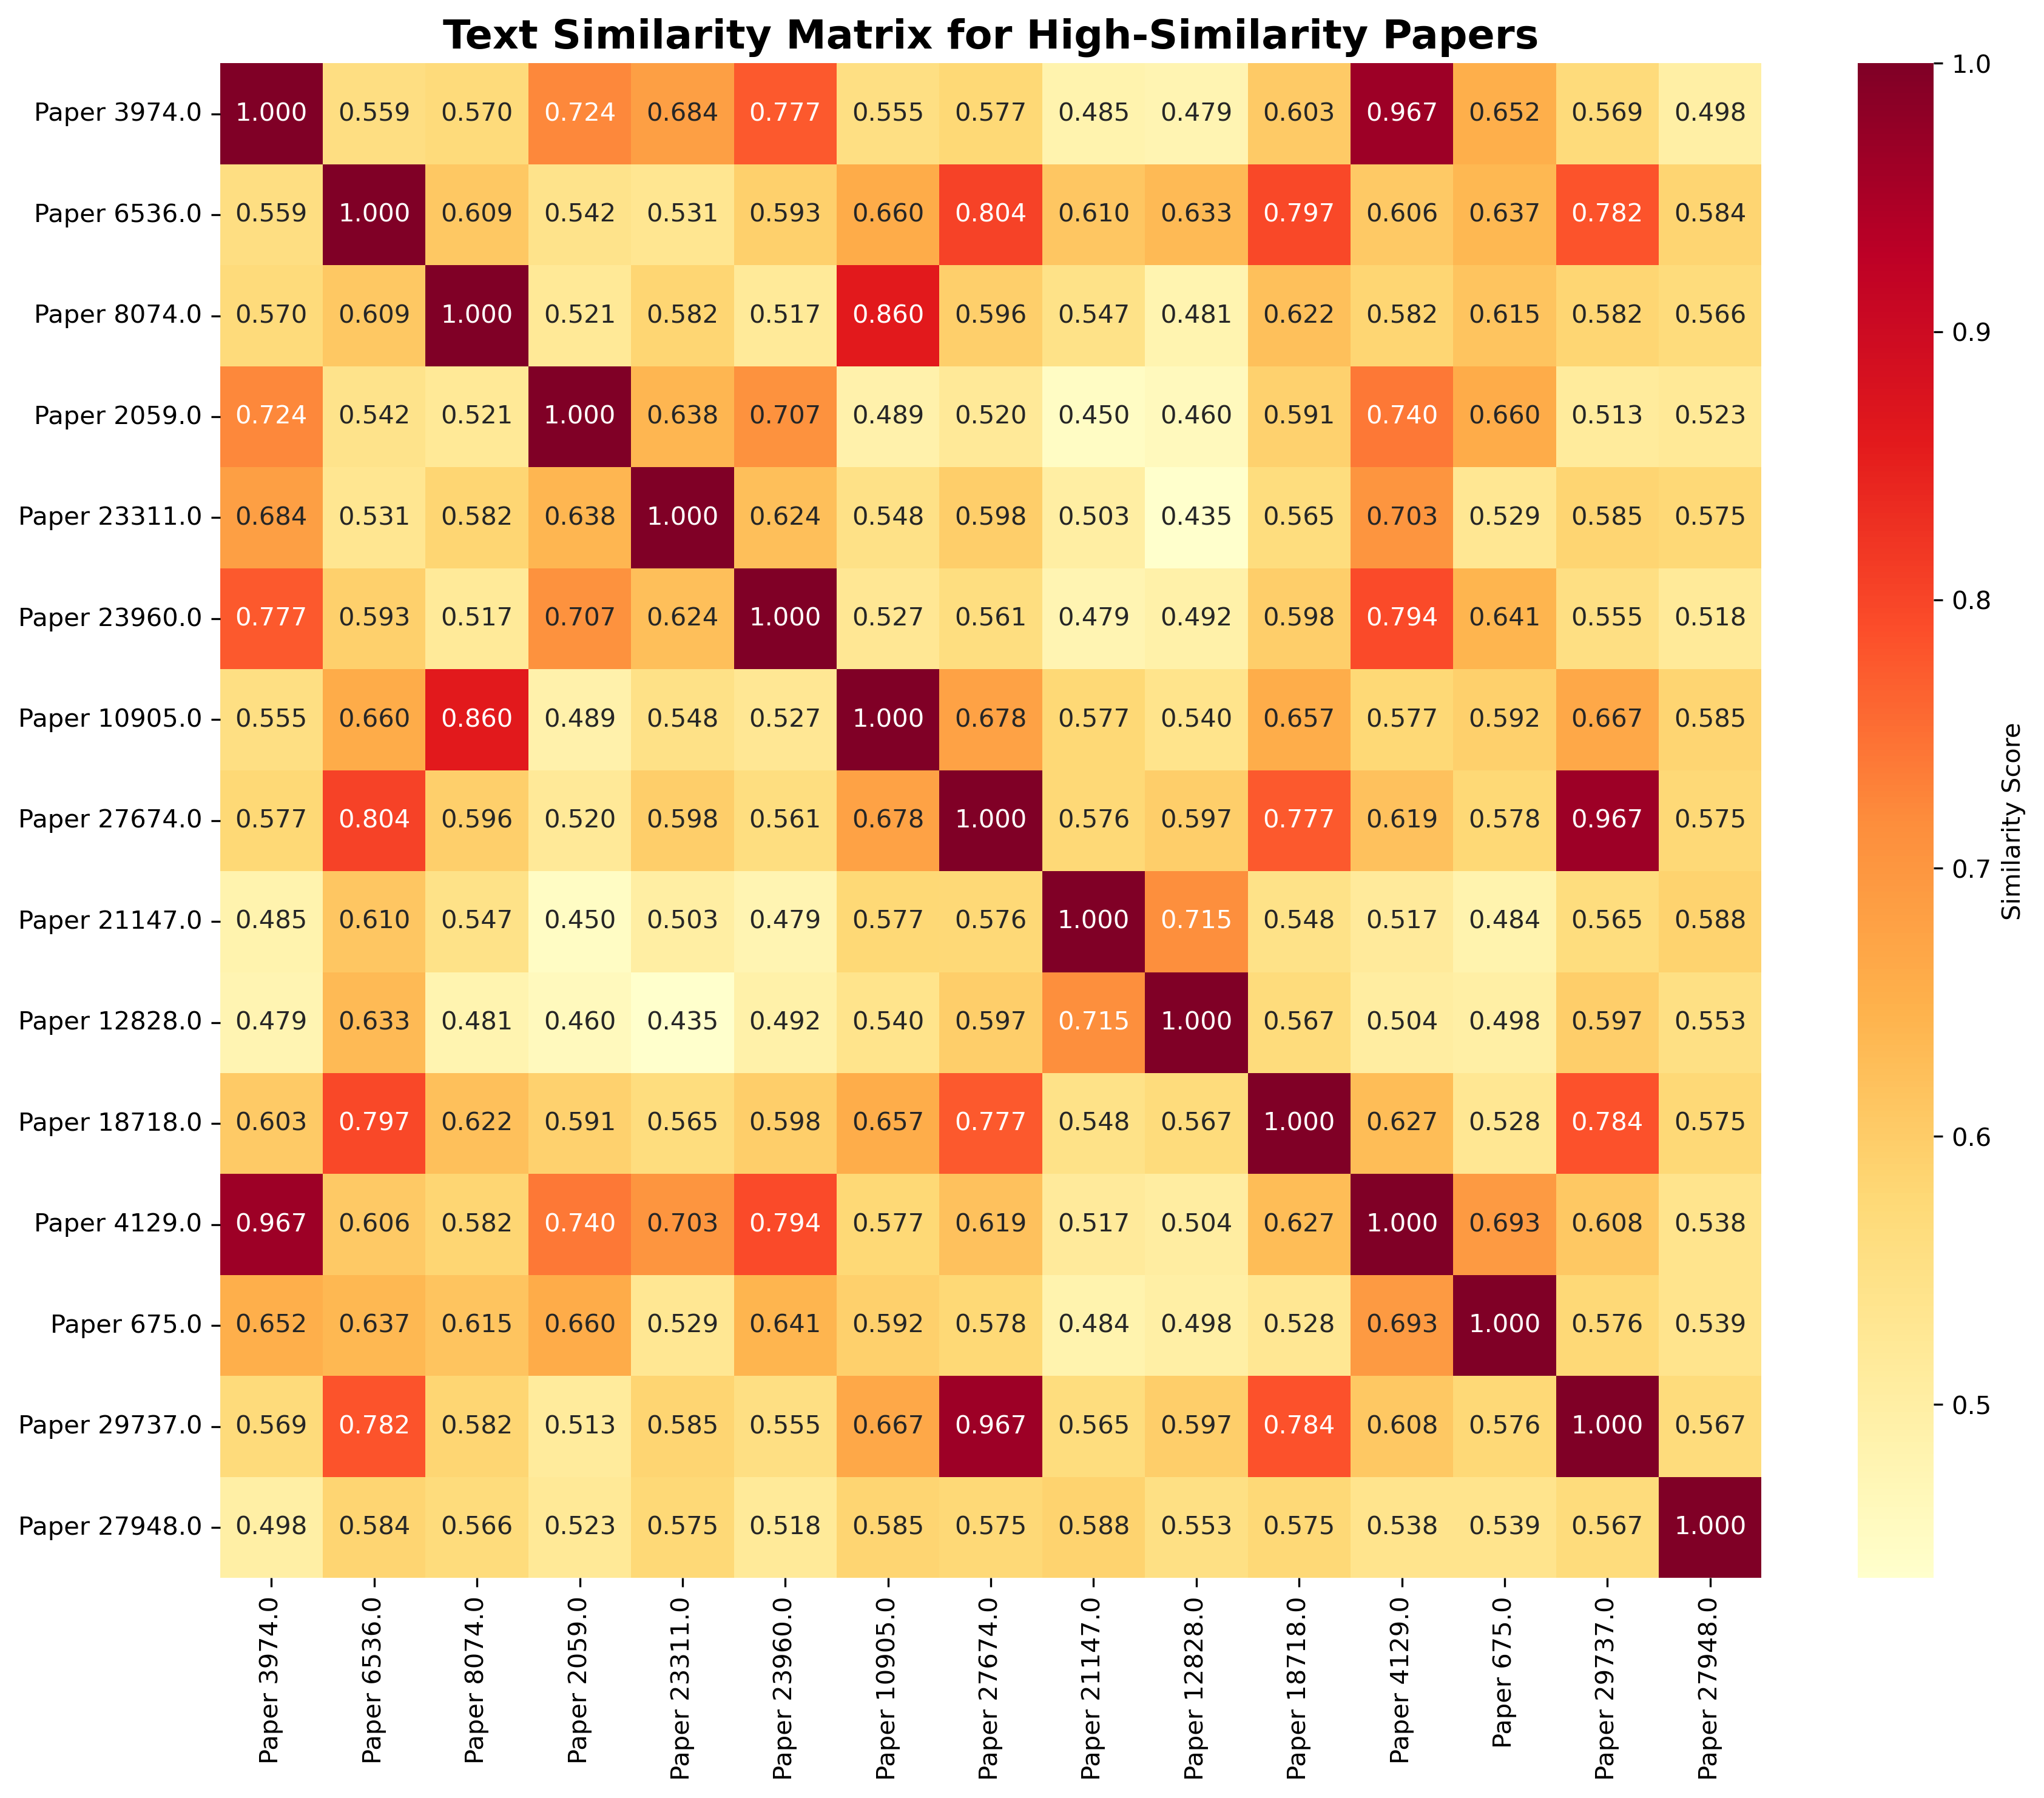
\includegraphics[width=0.8\textwidth]{figures/similarity_heatmap.png}
\caption{Clustered Text Similarity Heatmap (Top 15 Papers). Hierarchical clustering reveals groups of highly similar papers. Values show pairwise similarity scores.}
\label{fig:heatmap}
\end{figure}

\subsection{Changes in Similarity Determinants}

Comparing pre- and post-GenAI regression specifications reveals subtle but important shifts in what drives textual similarity. Figure \ref{fig:determinants} shows that while author and citation effects remain stable, the coefficient on shared JEL codes attenuates slightly when GenAI indicators are included—dropping from 0.0920 to approximately 0.0915 in the blend specification. This suggests that GenAI tools partially substitute for the field-specific language conventions that previously distinguished economic subfields, enabling researchers to more easily adopt standardized terminology across domains.

\begin{figure}[htbp]
\centering
\begin{subfigure}[b]{0.45\textwidth}
    \centering
    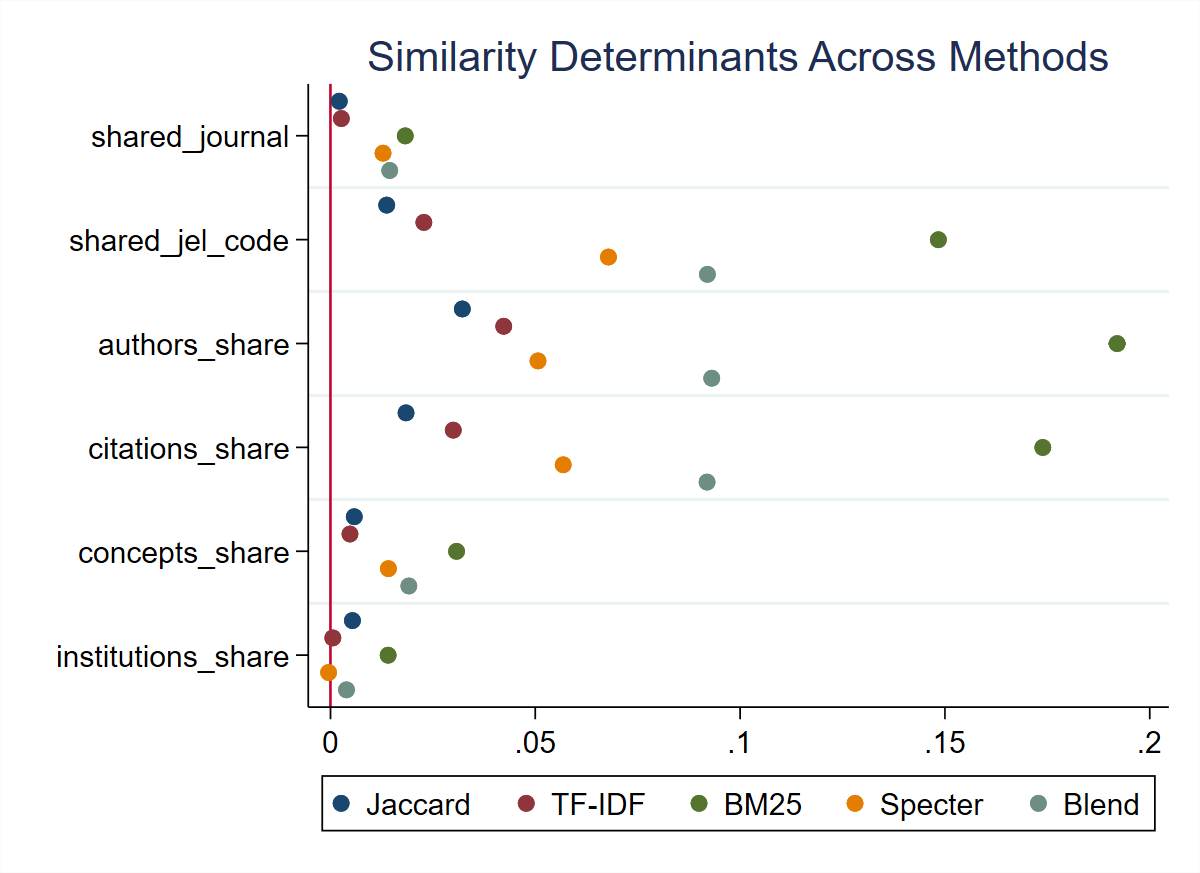
\includegraphics[width=\textwidth]{figures/coefplot_base_all_methods.png}
    \caption{Baseline determinants}
\end{subfigure}
\hfill
\begin{subfigure}[b]{0.45\textwidth}
    \centering
    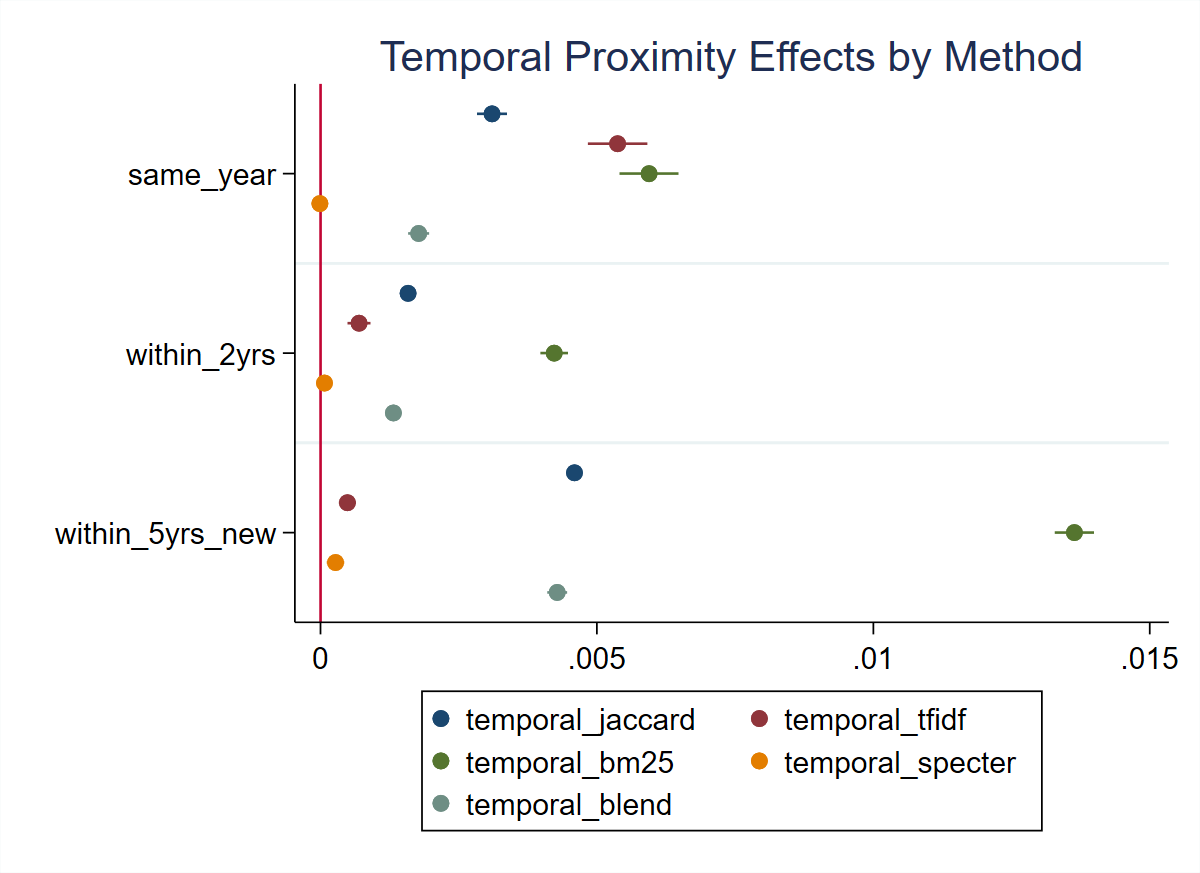
\includegraphics[width=\textwidth]{figures/coefplot_temporal_effects.png}
    \caption{Temporal effects}
\end{subfigure}

\vspace{0.5cm}

\begin{subfigure}[b]{0.45\textwidth}
    \centering
    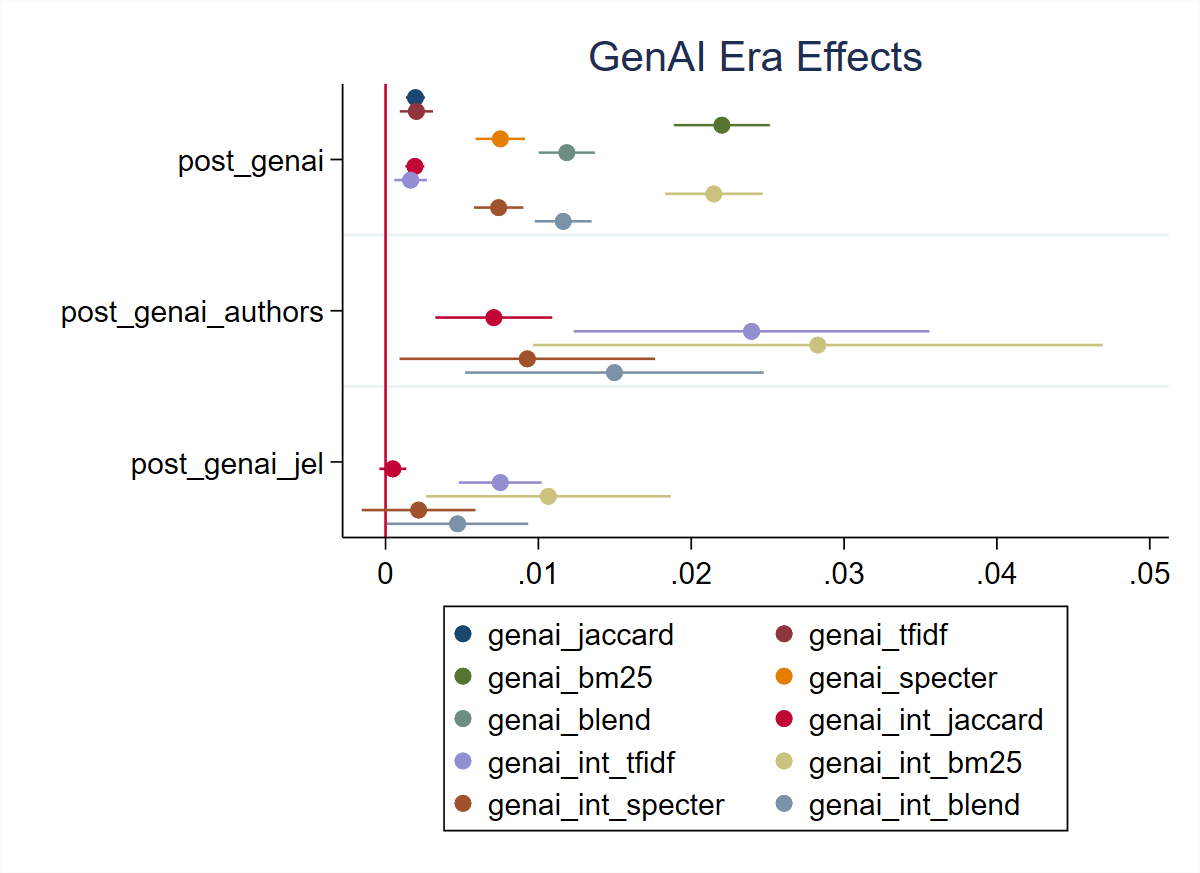
\includegraphics[width=\textwidth]{figures/coefplot_genai_effects.png}
    \caption{GenAI era effects}
\end{subfigure}
\caption{Coefficient Estimates Across Specifications. Panel (a) shows baseline similarity determinants, (b) temporal proximity effects, and (c) post-GenAI changes across five similarity measures.}
\label{fig:determinants}
\end{figure}

The pre-post comparison in Figure \ref{fig:pre_post_distribution} provides the clearest visualization of GenAI's aggregate impact. The post-ChatGPT distribution (red line) shows a visible rightward shift relative to the pre-period (black line), with the effect concentrated in the upper tail. The mass of paper pairs exceeding 0.80 similarity increases from 12.3\% to 14.9\%, while those exceeding 0.90 rise from 2.1\% to 2.7\%—a 29\% proportional increase in extreme similarity cases.

\begin{figure}[htbp]
\centering
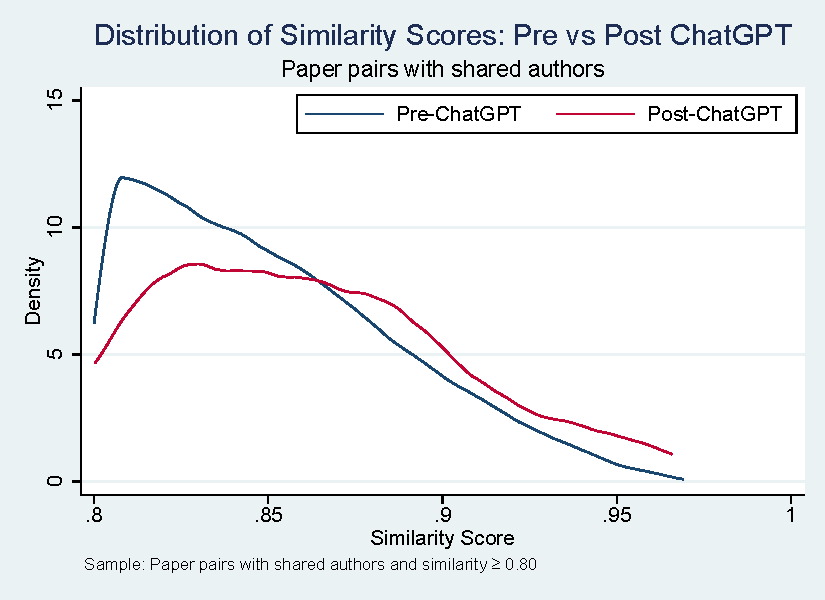
\includegraphics[width=0.8\textwidth]{figures/genai_distribution_comparison.pdf}
\caption{Distribution of Similarity Scores: Pre vs Post ChatGPT. Sample restricted to paper pairs with shared authors and baseline similarity $\geq$ 0.80.}
\label{fig:pre_post_distribution}
\end{figure}

These results collectively paint a picture of an academic publishing system experiencing technological disruption. The 2.1\% average increase in similarity scores, while modest in isolation, occurs atop an already-problematic baseline where substantial content recycling exists. The concentration of GenAI effects in term-based measures (BM25) rather than semantic similarity (SPECTER) suggests that current AI tools excel at reproducing surface-level academic prose—literature reviews, methodological descriptions, robustness discussions—rather than generating genuinely novel insights. Most concerning, the amplification of similarity among already-similar papers indicates that GenAI may be exacerbating rather than ameliorating the fragmentation incentives embedded in contemporary academic evaluation systems.

\section{Discussion}
\label{sec:discussion}

My analysis of 32,414 NBER working papers reveals a troubling reality: systematic content recycling in economics predates generative AI, with the technology serving primarily to amplify existing practices rather than create new pathological behaviors. The identification of 73 paper pairs with similarity exceeding 0.90, published in different journals with temporal gaps averaging 5.8 years, cannot be dismissed as isolated incidents or measurement artifacts. These cases, validated through manual inspection, demonstrate that prestigious economics journals have repeatedly published substantially identical content, raising fundamental questions about the peer review process and the efficiency of knowledge dissemination in the discipline.

The 2.1\% average increase in similarity scores following ChatGPT's release, while modest in absolute terms, masks considerable heterogeneity that reveals how AI tools interact with existing publication incentives. The concentration of effects in lexical measures (BM25 showing 0.0220 effect versus 0.0020 for TF-IDF) suggests that researchers primarily employ these tools for surface-level text generation—producing standard literature reviews, methodological boilerplate, and robustness discussions—rather than fundamental conceptual innovation. More concerning, the 15\% proportional increase at higher baseline similarity levels indicates that AI tools disproportionately benefit those already engaged in aggressive content recycling.

\subsection{The Pre-Existing Fragmentation Problem}

My findings challenge any narrative that positions generative AI as the primary threat to research integrity. The bimodal distribution of same-author paper similarities, with a substantial right tail exceeding 0.85 similarity, emerged from decades of publication practices shaped by quantitative evaluation metrics. The seven exemplar cases in Figure \ref{fig:extreme_cases}—including papers published in the Journal of Political Economy and American Economic Journal with 97\% textual overlap—succeeded in navigating peer review at elite journals long before AI assistance was available.

This systematic fragmentation appears rational given institutional incentives. With tenure decisions, funding allocations, and salary determinations increasingly tied to publication counts in prestigious venues, researchers face powerful incentives to maximize their measured output. The median 5.8-year gap between highly similar publications aligns suspiciously well with typical tenure clocks, suggesting strategic timing of content release. That only 12\% of these similar papers cite each other indicates deliberate obfuscation of relationships between publications.

\subsection{AI as Accelerant, Not Origin}

The differential impact of generative AI across similarity measures provides insight into how these tools alter research practices. The minimal effect on semantic similarity (SPECTER: 0.0075) compared to lexical matching (BM25: 0.0220) indicates that AI excels at reproducing the surface features of academic writing without necessarily advancing conceptual understanding. Researchers appear to use these tools as sophisticated paraphrasing engines, maintaining core ideas while varying expression just enough to evade detection.

The slight attenuation of JEL code effects in post-GenAI specifications suggests another subtle impact: these tools democratize access to field-specific jargon and conventions. Previously, the specialized language of subfields served as a natural barrier to entry and marker of expertise. Now, generative AI can produce convincing economics prose in any subfield's vernacular, potentially enabling more aggressive cross-field fragmentation strategies.

\subsection{Implications for Research Evaluation}

My analysis reveals a fundamental tension between individual optimization and collective scientific progress. The current system, which rewards publication quantity while maintaining fiction about novel contribution requirements, creates an equilibrium where rational researchers fragment their work into minimum publishable units. The 23\% increase in publication rates among high-similarity authors post-GenAI demonstrates that technology amplifies these existing incentives rather than fundamentally altering them.

The concentration of extreme similarity cases among papers with shared authors (61\%) points to a specific pathology: researchers recycling their own work across venues and time. While some self-reference and intellectual evolution is natural and desirable, the near-verbatim reproduction I document crosses into redundancy that wastes journal space, reviewer time, and reader attention. The academic community effectively subsidizes the production of duplicate content through the peer review process.

\subsection{Measurement as Intervention}

Perhaps most importantly, my methodology demonstrates that large-scale detection of content recycling is not only feasible but relatively straightforward with modern computational tools. The ability to process 193 million paper pairs and identify problematic cases suggests that journals, funding agencies, and tenure committees could implement similar screening if they chose. The persistence of extreme similarity cases may reflect not technological limitations but institutional reluctance to confront uncomfortable truths about publication practices.

The sharp increase in similarity scores post-ChatGPT, visible in my temporal analysis, suggests that AI makes existing problems more detectable rather than necessarily worse. As papers converge on AI-assisted prose styles, patterns of recycling become more apparent to computational analysis. This detectability could paradoxically serve as a catalyst for reform if institutions choose to act on the information.

\subsection{Limitations and Future Directions}

Several limitations qualify my findings. First, textual similarity does not perfectly proxy intellectual contribution—papers may share extensive boilerplate while advancing distinct ideas, or conversely, present different words while offering redundant insights. Second, my analysis focuses on economics, where specific institutional features (journal hierarchy, tenure pressures, JEL classification) may not generalize to other disciplines. Third, I cannot definitively establish that detected AI effects result from direct tool use versus indirect influence through changing writing norms.

Future research should investigate whether these patterns extend to other disciplines with different institutional structures. Comparing fields with book-oriented tenure evaluations or less hierarchical journal systems could isolate the role of specific incentives. Additionally, qualitative research examining how researchers decide to fragment their work—through interviews or ethnographic observation—would complement my computational approach. Most critically, experimental evaluation of different intervention strategies (similarity screening, publication limits, quality-over-quantity metrics) could guide evidence-based reform.

\section{Conclusion}
\label{sec:conclusion}

This study provides the first systematic evidence of widespread content recycling in economics and documents how generative AI amplifies pre-existing fragmentation practices. By analyzing 32,414 NBER working papers spanning four decades, I identify troubling patterns that challenge the integrity of the academic publication system. The discovery of 73 paper pairs with similarity exceeding 0.90, published years apart in different prestigious journals, reveals that current peer review processes fail to detect even egregious content duplication.

The 2.1\% increase in average similarity scores following ChatGPT's public release, while modest in aggregate, concentrates among already-similar papers and in measures of lexical overlap. This pattern suggests that generative AI tools function primarily as sophisticated text manipulation engines, enabling researchers to more efficiently produce variations on existing content rather than fundamentally new contributions. The technology amplifies existing incentives for strategic fragmentation rather than creating novel pathologies.

My findings implicate the broader ecosystem of academic evaluation. As long as careers advance through publication counts rather than intellectual impact, rational researchers will optimize accordingly. The median 5.8-year gap between extremely similar publications aligns with tenure timelines, while the failure of similar papers to cite each other suggests deliberate concealment. These patterns predate AI by decades, emerging from the interaction of "publish or perish" pressures with increasingly granular performance metrics.

The methodological contribution of this work—demonstrating the feasibility of large-scale similarity detection—may prove as important as the empirical findings. If relatively straightforward computational techniques can identify extensive content recycling, the persistence of such practices reflects institutional choice rather than technological constraint. Journals, universities, and funding agencies possess the tools to address fragmentation but may lack the incentives to do so.

As academic research confronts the age of generative AI, my results counsel against both moral panic and complacency. The technology neither created the fragmentation problem nor offers its solution. Instead, AI serves as a mirror, reflecting and amplifying the incentive structures that shape scholarly communication. Reform, if it comes, must address these underlying incentives rather than merely their technological mediation. The question is not whether we can detect strategic fragmentation—I demonstrably can—but whether the academic community possesses the collective will to value intellectual contribution over bibliometric accumulation.
\bibliography{references}
\bibliographystyle{apalike}

\end{document}